\chapter{Administrators}
There are two types of accounts in Obidos. One is administrative accounts and the other is user accounts.
An administrator account is used to manage Obidos. This includes managing administrative accounts, managing user accounts, setting up preferences, managing license, managing audits, etc.
An Administrator (herienafter referred to as admin) cannot store digital artifacts in Obidos.
An admin cannot assume the role of a user and a user cannot assume the role of an admin.
All admin accounts are local accounts. This means those accounts are maintained within Obidos.
Local accounts will have their passwords set according to the password policy in Obidos.

Obidos has a built-in admin account 'admin'.
The password for this account is set at the time of installation.
Using this 'admin' account additional admin accounts can be created.
The built-in 'admin' account inherits every capability that is possible for an administrative account. 
Such an account is referred to as a 'root admin'. The 'admin' account can be used to create other root admin accounts or less capable admin accounts.
\textcolor{myblue}{If your institutional security policiy requires renaming the default 'admin' account,
that can be done at the time of installation.}
Admin account operations are described in the sections to follow.

\section{License and number of users}
Obidos license is based on number of users. Only the count of active regular user accounts is considered for license units.
Admin accounts do not count towards license. So if there are 112 active regular user accounts and 7 admin accounts, only the 
112 user accounts are counted for license units. Once the active number of regular users reach the license limit, no new users can be
added by admins.

The Open Source license allows unlimited users and has no expiration.

\section{Create Administrators}
To create an admin account, log into Obidos using the 'admin' account (or another admin account).
From the "Admin Accounts" top navigation menu, select "Create New Admin".
The password assigned to this admin account during the account creation process is a temporary password.
The admin user will have to change the password when logging into Obidos for the first time.

\begin{figure}[H]
\centering
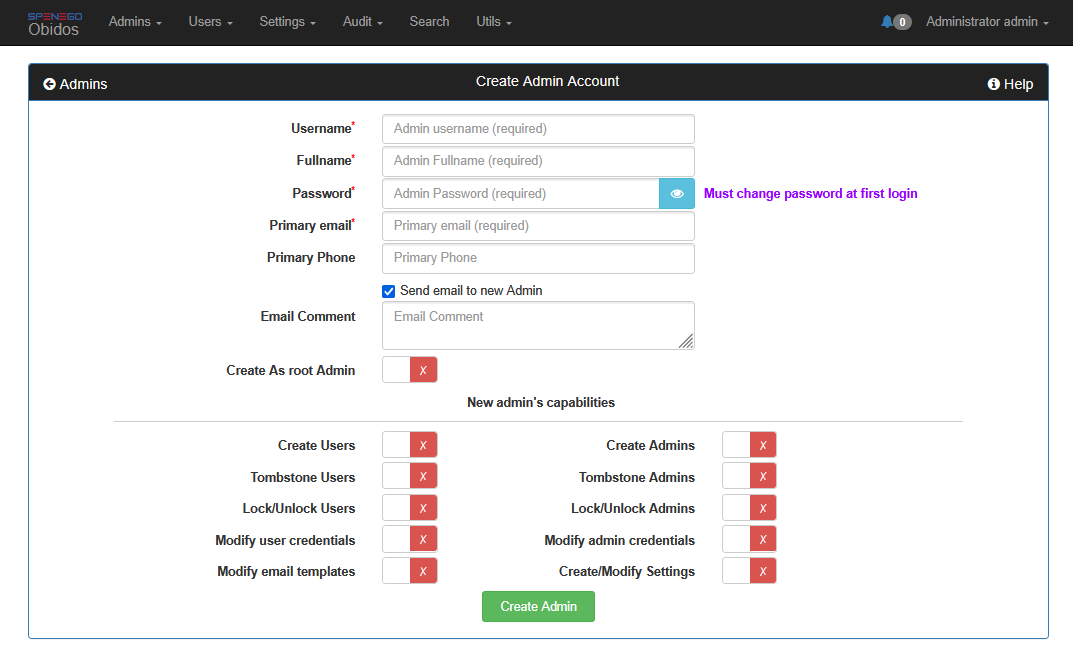
\includegraphics[width=90mm]{admin/Create-New-Admin.png}
\caption{Create New Admin Account}
\label{fig: Figure}
\end{figure}

\section{List Administrators}
Log into Obidos using an admin account.
From the "Admin Accounts" top navigation menu, select "List Admins".

\begin{figure}[H]
\centering
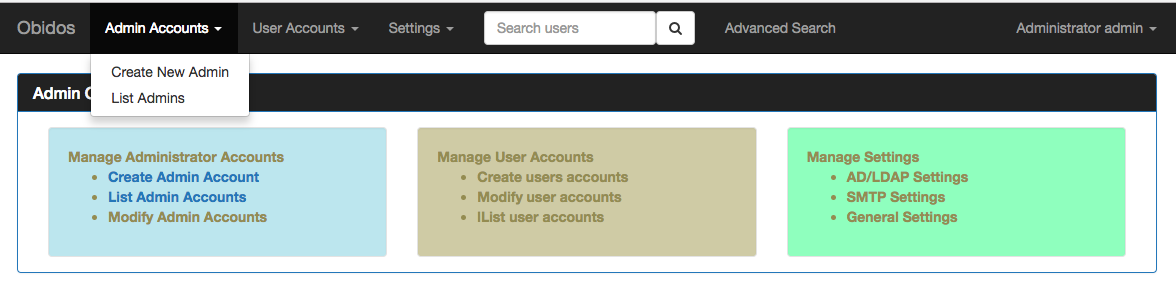
\includegraphics[width=90mm]{admin/Admin-Menu.png}
\caption{Admin Accounts Menu}
\label{fig: Figure}
\end{figure}

\section{Edit Administrator}
If the Fullname, Primary email, Primary phone number, or password has to be changed, it can be done
by editing the profile.
To get to the "Edit" task, first the admins must be listed.
This can be done by selecting "List Admins" from the "Admin Accounts" top navigation menu.
From the list of admins, click on the "Edit" button. This will open up an edit window.

\section{Delete Administrator}
Accounts can only be 'tombstoned' or 'locked'. They cannot be deleted.
Only a root admin account can be used to tombstone another administrator account.
The built-in 'admin' account cannot be deleted.
Once an admin account is tombstoned, the whole profile associated with that account will be frozen.
To get to the "Tombstone" task, first the admins must be listed.
This can be done by selecting "List Admins" from the "Admin Accounts" top navigation menu.
From the list of admins, select the admin(s) of interest click on "Tombstone" button.
A confirmation pop-up window will show up. Select "Yes" to confirm or "No" to cancel.
